\section{Testing}
The driver's job is to send commands from the Bluez stack to the device and get back its response. If all of this happens successfully then that should mean that the BlueNRG is able to communicate with another device using some BLE use cases.\\
Some of the use cases that can be used to test this are:
\subsection{Checking to see if BLE gets enabled} 
	\begin{enumerate}
		\item This can be done using the following command\\
			\textbf{sudo hciconfig hci0 lestates}
		\item This command should return the following output:
			\begin{figure}[ht]
			\centering
			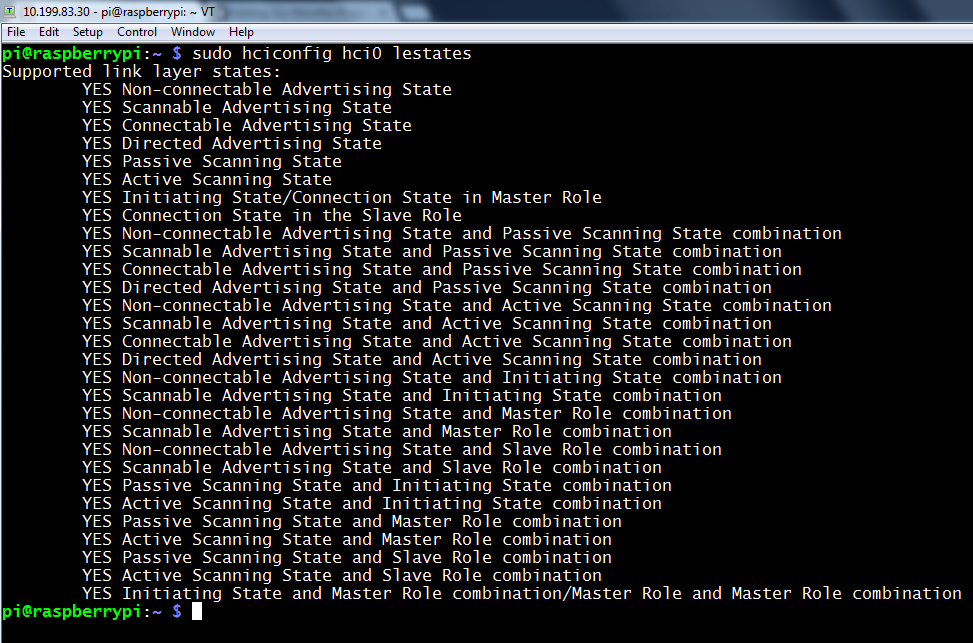
\includegraphics[scale=0.5]{images/lestates.png}
			\caption{List of LE states supported by adapter}
		\end{figure}
	\end{enumerate}
\subsection{BLE gatttool interaction} 
gatttool is one of the best methods to interact with another BLE device interactively from a Linux host. It opens an interactive session.
	\begin{enumerate}
		\item Find out the MAC\_ADDR of the other device using\\
			\textbf{sudo hcitool lescan}
			\begin{figure}[ht]
				\centering
				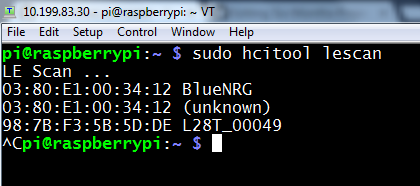
\includegraphics[scale=0.5]{images/lescan.png}
				\caption{List of LE devices scanned}
			\end{figure}
		\item Open interactive session using gatttool:\\
			\textbf{sudo gatttool -i hci0 -b MAC\_ADDR -I}
		\item In the interactive sesssion type in the following commands:\\
			\textbf{connect}
		\item Read profiles:\\
			\textbf{primary}
		\item Read all available characterstics:\\
			\textbf{char-desc}
			\begin{figure}[ht]
				\centering
				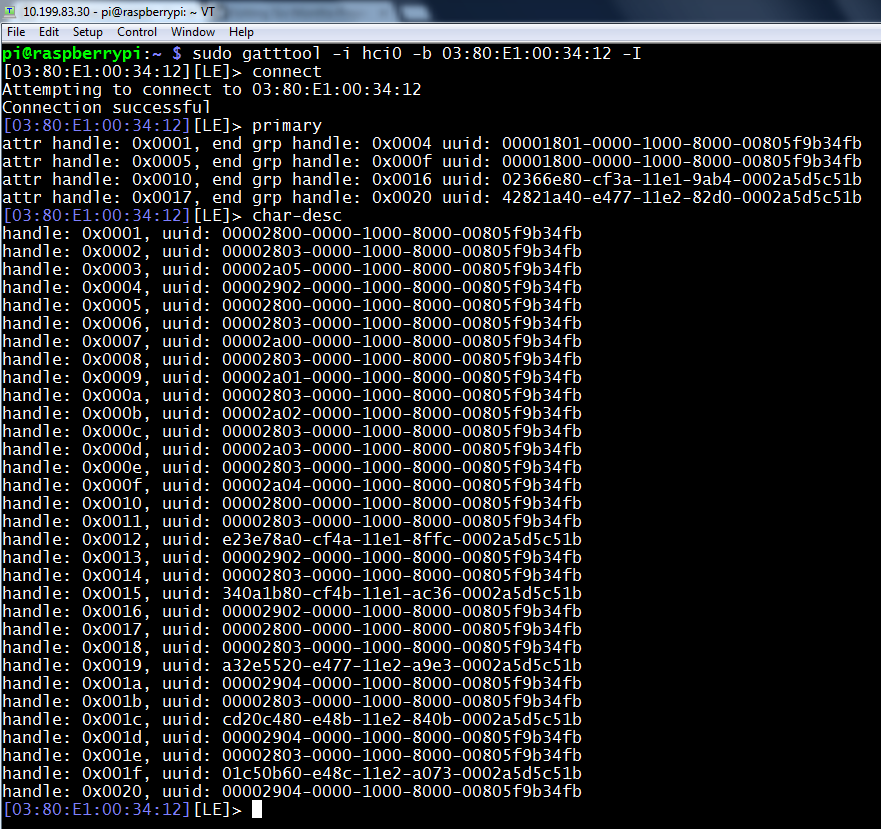
\includegraphics[scale=0.5]{images/gatttool1.png}
				\caption{GATTtool interaction part-I}
			\end{figure}
		\item Read the value of a characterstic:\\
       			\textbf{char-read-hnd The\_characterstic\_handle}
   			\item Write to a particular characterstc:\\
       			\textbf{char-write-cmd handle Value\_in\_Hex}
				\begin{figure}[ht]
				\centering
				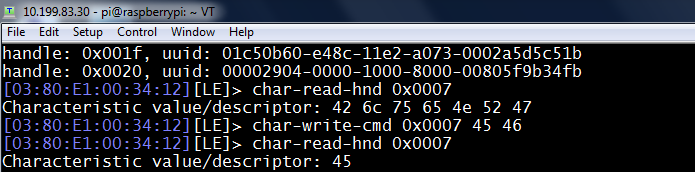
\includegraphics[scale=0.5]{images/gatttool2.png}
				\caption{GATTtool interaction part-II}
			\end{figure}
   			\item Disconnect:\\
       			\textbf{disconnect}
   			\item Quit:\\
       			\textbf{quit}
	\end{enumerate}
\subsection{Reading Beacons using BLE}
	\begin{enumerate}
		\item There is a python script that can be used for this purpose, install it:\\
			\textbf{git clone https://github.com/switchdoclabs/BeaconAirPython.git}
		\item In order to use, the following package must be installed:
			\textbf{sudo apt-get install python-bluez}
		\item Scan and Read the beacons:\\
			\textbf{cd BeanconAirPython/ble}\\
			\textbf{sudo python testblescan.py}
		\item This should list out the nearby beacons:
			\begin{figure}[ht]
				\centering
				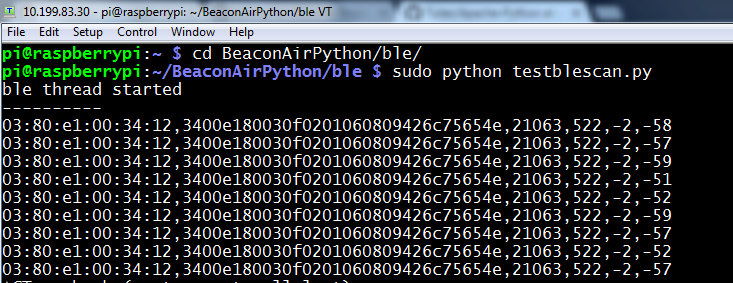
\includegraphics[scale=0.5]{images/beacon_read.png}
				\caption{Reading beacons}
			\end{figure}
	\end{enumerate}
\subsection{Advertising with Beacons}
	\begin{enumerate}
		\item Start advertising in non-connectable state:\\
			\textbf{sudo hciconfig hci0 leadv 3}\\
			\textbf{sudo hciconfig hci0 noscan}
		\item Broadcast a beacon:\\
			\textbf{sudo hcitool -i hci0 cmd 0x08 0x0008 1E 02 01 1A 1A FF 4C 00 02 15 63 6F 3F 8F 64 91 4B EE 95 F7 D8 CC 64 A8 63 B5 00 00 00 00 C8}
		\item You should see the following as output:
			\begin{figure}[ht]
				\centering
				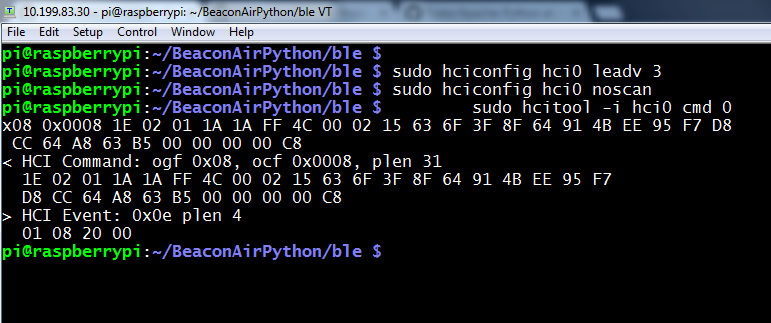
\includegraphics[scale=0.5]{images/advertising_beacons.png}
				\caption{Advertising using beacons}
			\end{figure}
	\end{enumerate}
